%%%%%%%%%%%%%%%%%%%%%%%%%%%%%%%%%%%%%%%%%%%%
% 石浦研究室 卒論・修論テンプレート 【門外不出】
% 2018-01-09: 卒論の表紙を変更
% 2017-11-28: 小規模更新
%%%%%%%%%%%%%%%%%%%%%%%%%%%%%%%%%%%%%%%%%%%%

\documentclass[11pt]{jbook}
\usepackage{ist-thesis}
\usepackage[dvips]{graphicx}
\usepackage{tabularx}
\thesistype{B}  % 卒業論文の場合
%\thesistype{M}  % 修士論文の場合

\ID{6627} % 学籍番号 (下4桁)

\author{藤本 高史} % 著者名
\supervisor{石浦 菜岐佐 教授} % 指導教員
\yearmonth{2020年3月} % 提出年月 (固定です)

% 表紙でタイトルを改行したい場合は \PAR を入れる (内容梗概で改行されない)
\title{機械学習を用いたファズデータの \PAR チェックサム及びハッシュ値の推定} % 邦題

% 英文のアブストラクトを書かない場合は下記は省略可能
%\eauthor{Taro Kwangaku} % 英著者名
%\etitle{English Title English Title\PAR English Title English Title} % 英題

\abstract{
% 内容梗概は改段落しないので, \par は削除してね
%本研究では〜を提案する/〜をした (卒論). 本論文では〜を提案する (修論).\par
%次に, 簡単な背景 (あるいは本研究が解決しようとしている課題) を一文で書く.\par
%具体的に何をしたか書く (冒頭の文と同じ内容を, より具体的に書けばよい).\par
%技術的なポイントとなることを 2〜3 項目, それぞれ一文で書く.\par
%最後に, 得られた結果を簡潔にまとめる.
本研究では, 機械学習を用いてデータのチェックサム及びハッシュ値の推定を行う手法を提案する.
正当又は不当なデータをソフトウェアに入力することによって, ソフトウェアの脆弱性のテストを行う変異ベースのファジング手法では, チェックサムやハッシュ値により入力データは殆ど通過しないため, 網羅率が低いという課題があげられる.
これに対し, 難波はニューラルネットワークによるチェックサムの推定を行ったが, 入力データが8 byteの固定長しか学習を行っていないため, 汎用性に欠ける.
これを解決するため, 本研究では8 byte以上の入力データに対するチェックサム及びハッシュ値の推定を行う.
%ディープラーニングを用いて, 文字列からチェックサム及びハッシュ値を推定を行った.
%入力データとなる文字列は, ランダム文字列と規則性のある文字列として英文を使用する.
%文字列の長さは可変長である.
機械学習を行うための学習モデルにEncoder・Decoderモデルを使用する.
Kerasを使用してニューラルネットワークの構築および学習を行った.
結果, チェックサムはランダム文字列に対して20\%, 英文に対して50.8\%, CRC16 はランダム文字列に対して9.01\%,
英文に対して50.8\%, CRC32はランダム文字列に対して11.9\%, 英文に対して4.17\%の正答率が得られた.
}

\keyword{機械学習, ニューラルネットワーク, ファジング, Encoder・Decoder, 変異ベース, チェックサム, ハッシュ}

%\eabstract{
%First paragraph. First paragraph. First paragraph.
%First paragraph. First paragraph. First paragraph.
%First paragraph. First paragraph. First paragraph.
%First paragraph. First paragraph. First paragraph.
%First paragraph. First paragraph. First paragraph.
%First paragraph. First paragraph. First paragraph.
%
%Second paragraph. Second paragraph. Second paragraph.
%Second paragraph. Second paragraph. Second paragraph.
%Second paragraph. Second paragraph. Second paragraph.
%Second paragraph. Second paragraph. Second paragraph.
%
%Third paragraph. Third paragraph. Third paragraph.
%Third paragraph. Third paragraph. Third paragraph.
%}
%
%\ekeyword{English, Abstract}

\begin{document}

\coverpage

\tableofcontents

\body

\chapter{序論}

近年, 様々なシステムやソフトウェアのプログラムに対するセキュリティは大きな注目を浴びている. プログラムやシステムの脆弱性が存在すると, 不具合が生じたり, 第三者からの攻撃によって様々な被害が出る恐れがある. これらの被害を防ぐため, プログラムやシステムには徹底的なテストが必然となっている.

その脆弱性を検出するテストの一手法にファジングと呼ばれる手法がある. 与えられたプログラムに対して, 本来想定されていない情報を大量に入力し, その入力に対する動作に異常がないかどうかをテストする.

ファジングで使用するデータの生成方法として変異ベース手法がある. 変異ベース手法は既存の入力データの文字列等に該当する部分を変化させて新たなテストデータを生成する手法である. 入力データの一部を変異させるため, テストデータの作成に時間はかからず汎用性も高いが, テストデータの質は低い. 特に, テスト対象のプログラムにデータ検査としてチェックサムやハッシュ値が存在すると, 破損データとして扱われ, 入力データ通過率が非常に低くなると言う課題がある.

その課題を解決するために, 難波\cite{namba}は, ニューラルネットワークを用いて入力データに対するチェックサムの学習及び推定を行い, 68\%の正答率が得られた. しかし, この学習済ニューラルネットワークは, 8 byteの固定長のデータに対するチェックサムのみを対応していないため, ファジングツールへ実装をすると, 実際に使用することができる場面がかなり限定的になってしまうので, 汎用性に欠けるという課題がある.

本研究では難波\cite{namba}の汎用性の向上を目的に, 8 byte以上の入力データに対するチェックサム及びハッシュ値の推定を行う.
推定にニューラルネットワークを使用し, 特に(Seq2Seq)Encoder・Decoderモデル\cite{seq2seq}を用いる.
入力データは可変長データで学習を行う.
推定する値としてチェックサム, CRC16\cite{crc}, CRC32\cite{crc}, MD5\cite{md5}, SHA1\cite{sha1}を採用する.
結果として, チェックサム及びCRC16\cite{crc}, CRC32\cite{crc} に対して高い精度の正答率が得られた.

以下, 2 章で難波\cite{namba}の内容と課題について説明し, 3 章でニューラルネットワークを用いたの課題克服方法について述べ, 4 章で実験内容と実験結果を述べ, 5 章で結論とする.

\chapter{ニューラルネットワークを用いた \\ チェックサムの推定}
\section{チェックサムとCRC及びハッシュ値}

チェックサムは誤り検出符号の一種であり, 特定の計算方法を用いて元になるデータから一定の計算手順により求められた, 規則性のない値のことである.
主にデータの検査をするために用いられる.

%指定した長さのデータの数値に全て加算処理を行い, 特定の整数の剰余の値となる.
データの検査を行うとき, 入力するデータ全体や分割したデータに対して計算を行い, その結果をデータに付加する.
そして, チェックサム及びハッシュ値を計算した算術と同じ方法で再度計算を行い, その値がデータの後ろに付加されている値と比較して一致するかどうか確認を行う.
一致していなければ, 検査したデータは破損したデータとして扱われる.

チェックサムの計算方法は, 対象となる文字列に対して各文字を全てASCIIコードに置き換え, それを合算した値から256の剰余をとる.
計算方法の例を図\ref{cksum}に示す.
図にあるThank you very much.という文字列のチェックサムを計算を行うとすると, 初めに各文字全てをASCIIコードに準拠した整数に置き換える.
そして, 置き換えた値を全て加算した値から256の剰余を行うことでチェックサムが得られる.
最後に, 文字列に計算したチェックサムを付加する.


\begin{figure}[htbp]
\begin{center}
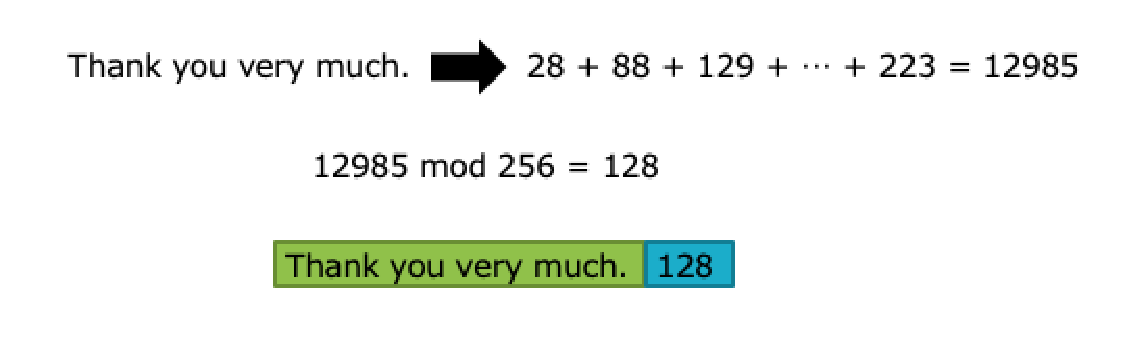
\includegraphics[width=130mm]{chsum.eps}
\caption{チェックサムの計算例}
\label{cksum}
\end{center}
\end{figure}

ハッシュ値は, ハッシュ関数から出力された規則性のない固定長のビット列である.
ハッシュ値の計算方法はハッシュ関数によって様々である.
ハッシュ値は一方向関数なため, ハッシュ値から元の文字列を特定することはできない.
その性質を利用して, 暗号などのセキュリティの分野で多く使用されている.

CRC\cite{crc}は誤り検出符号の一種であり, データから特定の定数の剰余を検査用の値として用いる.
主にPNGやZIPなどのファイルのデータ検査や, HDLC手順やCSMA/CD方式などの誤りチェック及びノイズチェック使われている.
出力されるbit 数はCRC\cite{crc}の種類によって異なる.
例えば, CRC16\cite{crc}であれば16 bit以下の2 進数が出力され, CRC32\cite{crc}では32 bit以下の2 進数が出力される.

MD5\cite{md5} 及びSHA1\cite{sha1} は暗号学的ハッシュ関数の一種であり, MD5\cite{md5} はデータを元に出力した128 bitの値, SHA1\cite{sha1} は160 bitの値を用いる.
出力されるbit数は, どんなデータでも必ず定められた固定長で出力される.
IPsec, SMTPなどのセキュリティープロトコルで使用されている他, 暗号や認証, デジタル署名などにも用いられている.

CRC\cite{crc}, MD5\cite{md5}, SHA1\cite{sha1}の出力値の例を図\ref{hash}に示す.
Helloという文字列からCRC16\cite{crc}を計算すると, 1 と0 の2 進数の値が出力される.
出力されるbit数が16 bit以下となるのは, CRCは特定の方程式から文字列を2 進数に表した値の剰余を出力とするためである.
Goodという文字列からMD5\cite{md5}, Niceという文字列からSHA1\cite{sha1} を計算すると, 0 $\sim$ Fの16 進数の値が出力される.
出力されるbit 数は, 必ず固定長である.

\begin{figure}[htbp]
\begin{center}
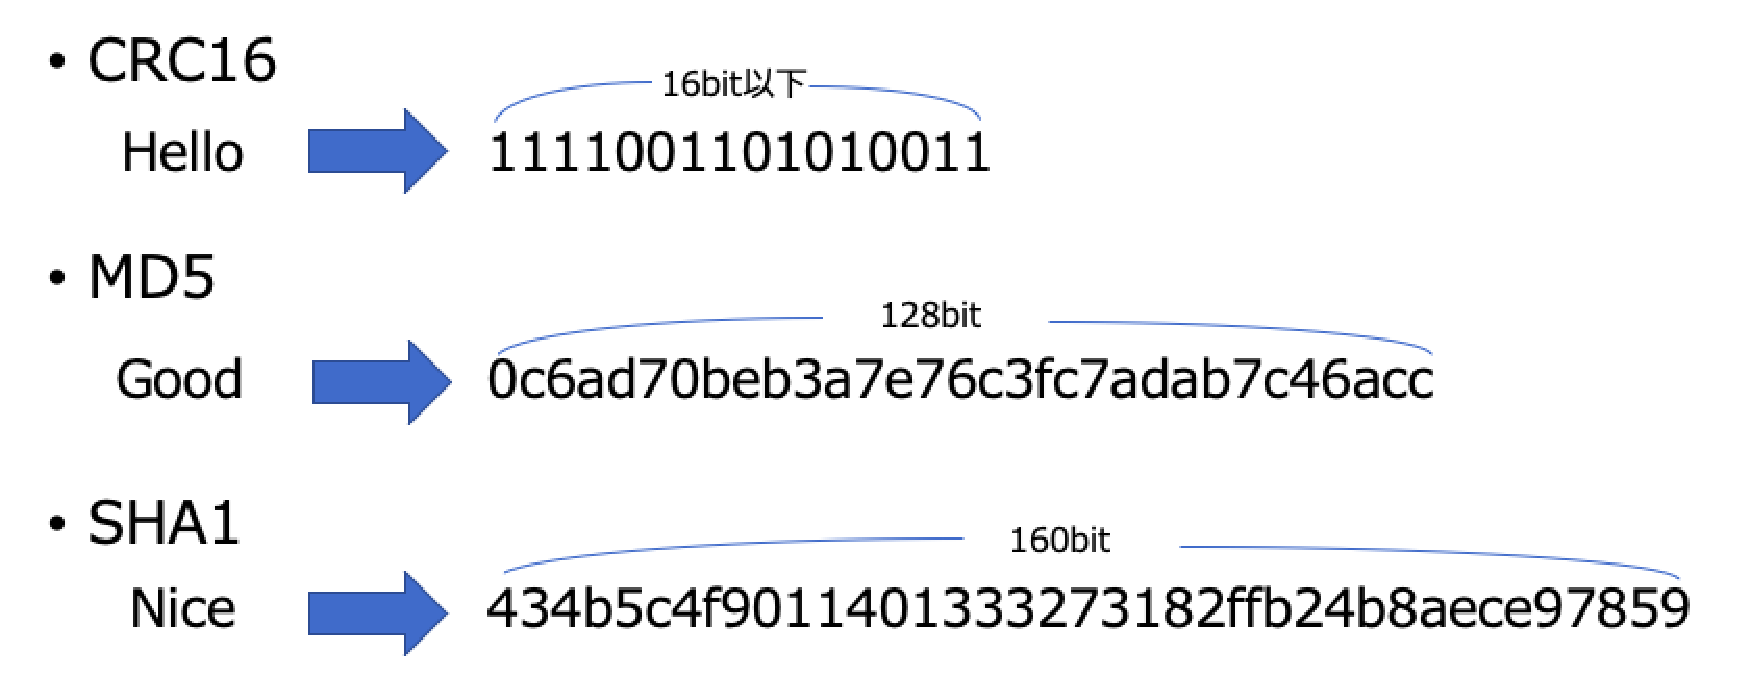
\includegraphics[width=130mm]{hash.eps}
\caption{CRC, MD5, SHA1のハッシュ値}
\label{hash}
\end{center}
\end{figure}


\section{ニューラルネットワークを用いたチェックサムの推定}

ニューラルネットワークはパーセプトロンのアルゴリズムを3 層にし, 誤差逆伝播法と呼ばれる学習機能を持たせた多層パーセプトロンである.
一般的なニューラルネットワークを図\ref{NN}に示す.
ニューラルネットワークは入力層, 中間層, 出力層の3 つの層で構成されている.
入力層は情報を入力するためのニューロンであり,入力層から情報を受け取った中間層は,情報を分析し, 学習した後にその結果を次の層のニューロンに繰り返し伝達させ,
最終的に出力層で結果が出力される.
そこで, ニューラルネットワークが予測した値と真理値を比較し, 誤差逆伝播により最適な重みへと更新していく.

\begin{figure}[htbp]
\begin{center}
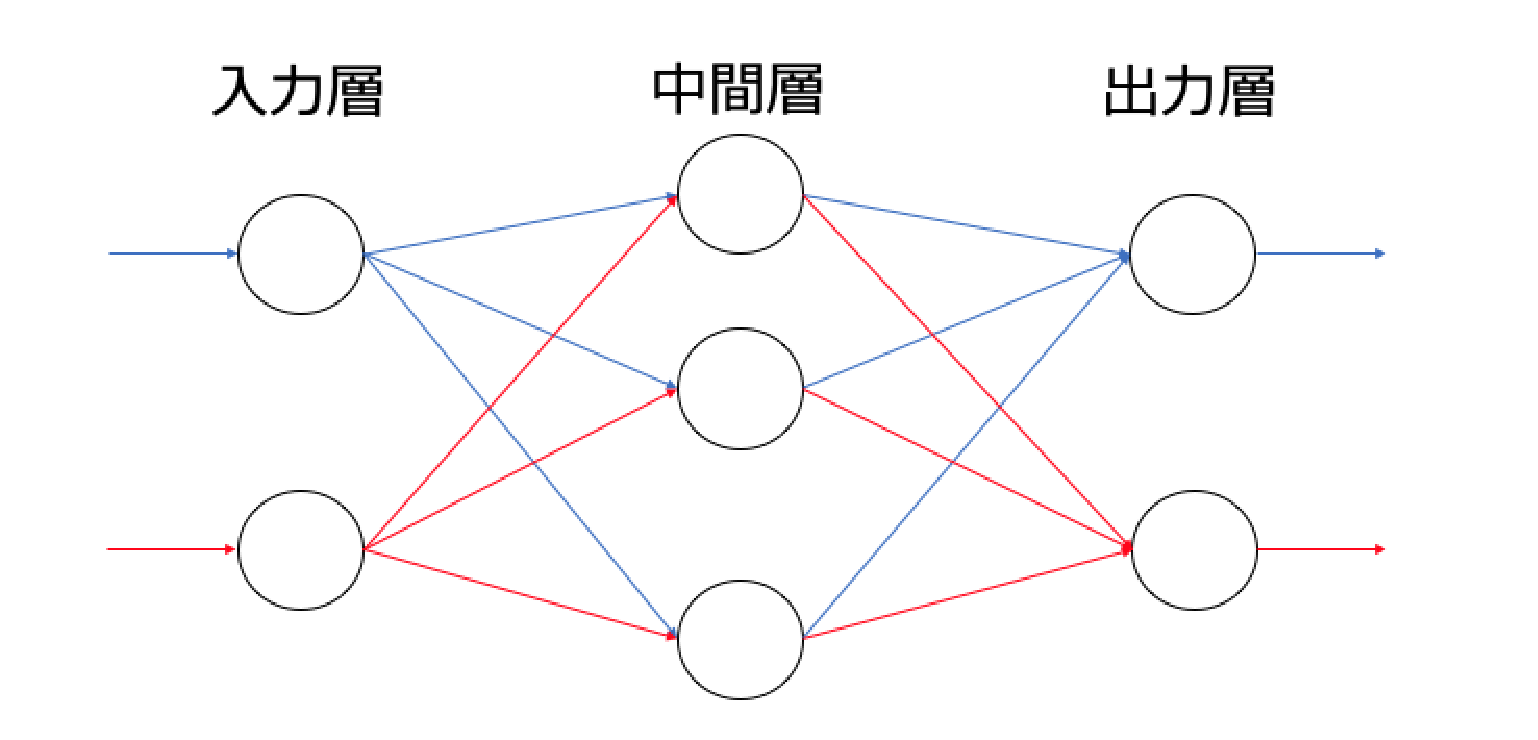
\includegraphics[width=80mm]{NN.eps}
\caption{ニューラルネットワーク}
\end{center}
\label{NN}
\end{figure}

RNN(Recurrent Neural Network)は, ニューラルネットワークの各層の出力を再度, その層の出力に
そのまま再帰するという特徴をもつニューラルネットワークである.
RNNの構成を図\ref{rnn}を以下に示す.
主に時系列データと呼ばれる時間的な順序に従って一定の感覚で集められたデータを分析, 計算するという役割をもつ.
層の構成として, 入力層, 中間層, 出力層となっているが, 中間層は過去の情報を保持する.
しかし, RNNは過去の情報を全て記憶した状態で計算を行うので, 計算量が多くなると共に,
計算に不要な情報までも取り入れてしまう欠点をもつ.

この欠点を解決したのがLSTMである.
LSTMの構成を図\ref{lstm}に示す.
中間層に入力ゲート, 忘却ゲート, 出力ゲートの3 つのゲートを利用して計算を行う.
この3 つのゲートはそれぞれ, 計算を行う上で何が必要で何が不必要なのか取捨選択をすることができる.


\begin{figure}[htbp]
\begin{center}
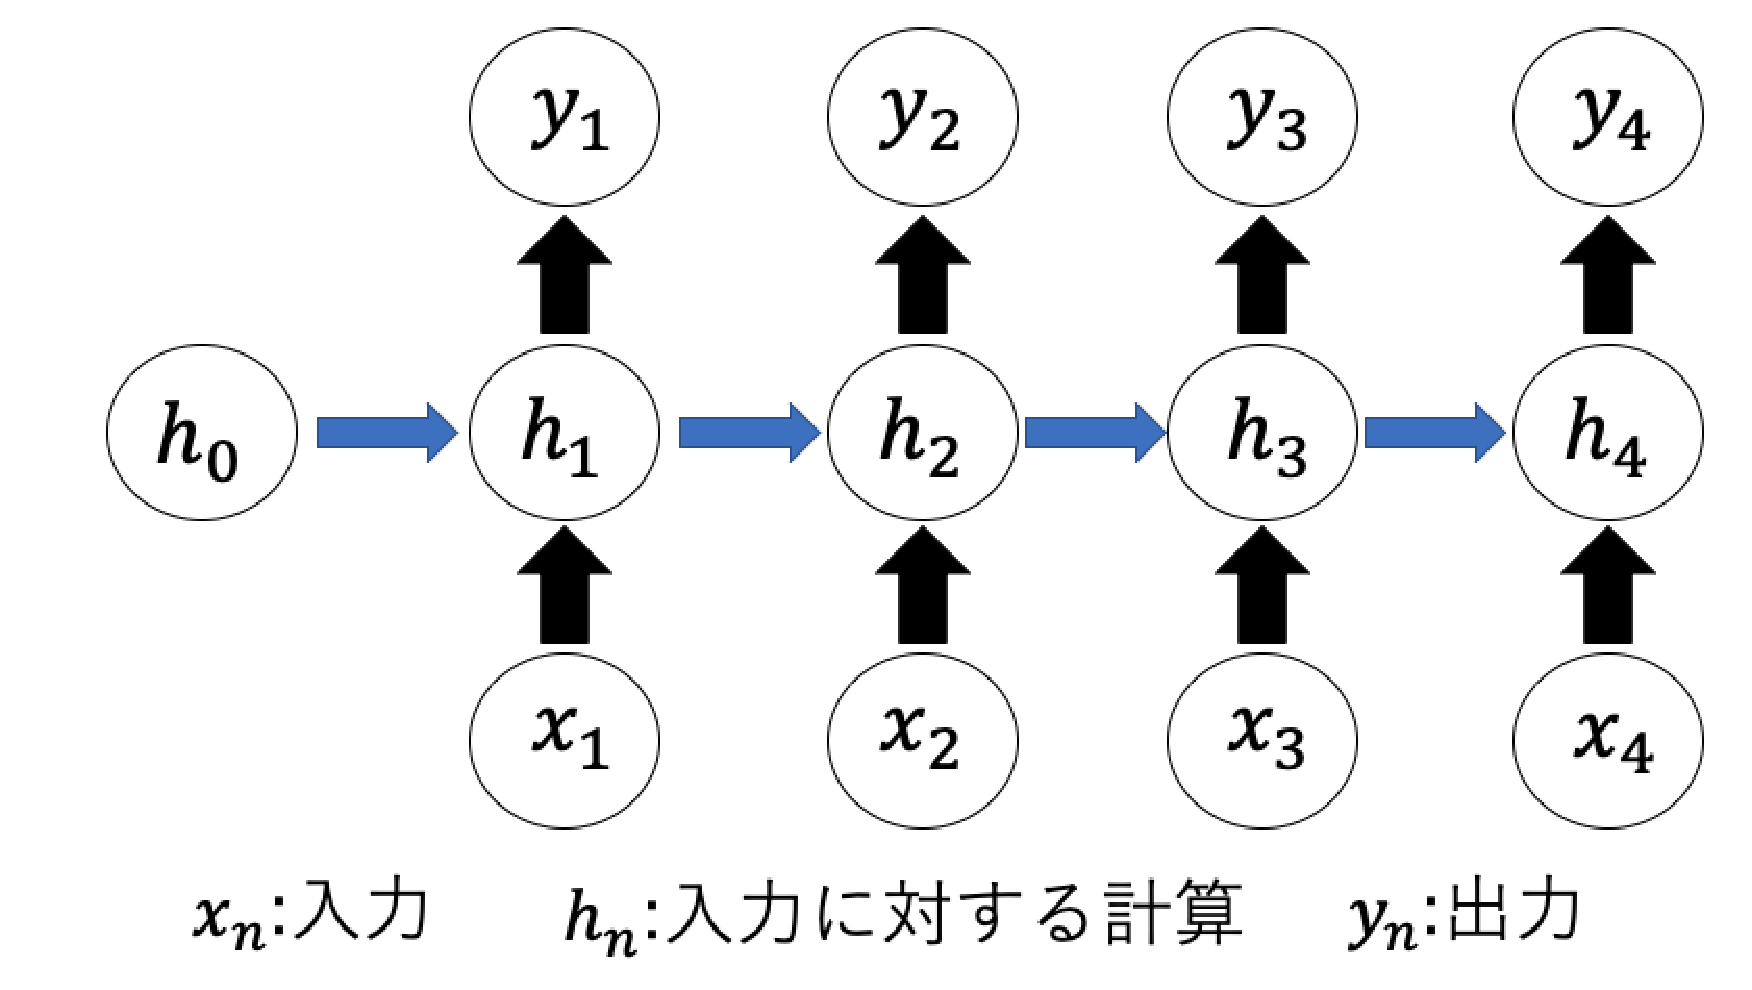
\includegraphics[width=80mm]{rnn.eps}
\caption{RNN}
\end{center}
\label{rnn}
\end{figure}

\begin{figure}[htbp]
\begin{center}
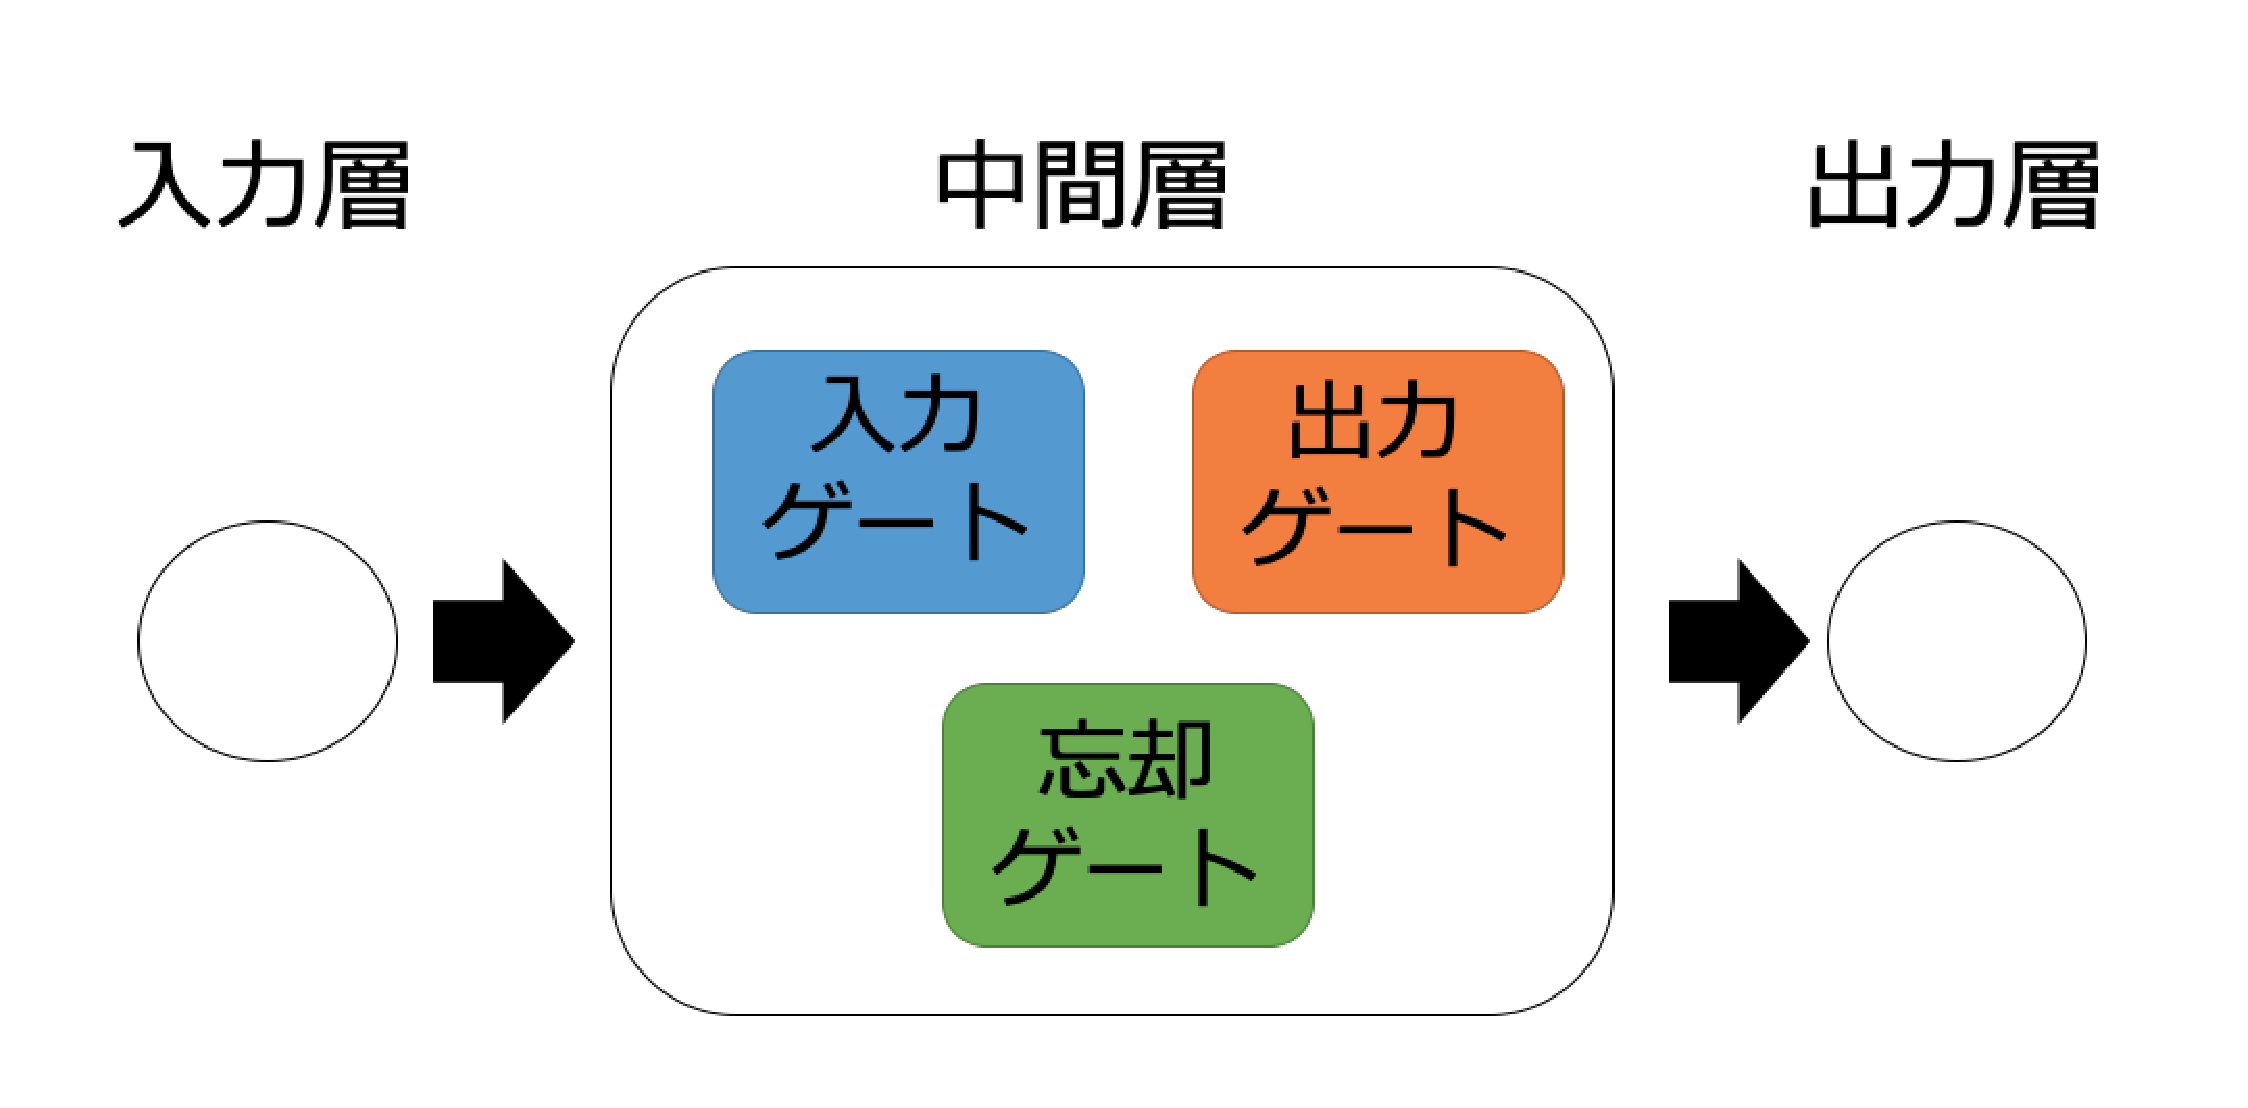
\includegraphics[width=80mm]{lstm.eps}
\caption{LSTM}
\label{lstm}
\end{center}
\end{figure}

難波\cite{namba}はニューラルネットワークを用いて, 8 byteの入力データに対するチェックサムの推定を行っている.
正規データからデータとチェックサムの集合を抽出し, ニューラルネットワークに学習させる.
学習済ニューラルネットワークで変異データからチェックサムを推定し, 更新する.
学習の仕組みを, 図\ref{hantei}に示す.
初めに, 文字列とその文字列に対するチェックサムのデータを用意する.
次に, そのデータをニューラルネットワークへ入力をし, 学習を行う.
そして, 学習済ニューラルネットワークに対して, 文字列を入力することにより, チェックサム及びハッシュ値を推定する.
最後に, 推定したチェックサムを, 文字列の末端に付与する.
よって, 正当な入力データとして扱われる.

難波\cite{namba}のニューラルネットワークの構造を図\ref{namba}に示す.
各層の数字はノード数を表す.
初めにランダム文字列から1つ1つの文字を分割して入力を行い, Embedding層で入力データのベクトル化を行う.
次にEmbedding層から受け取った情報を元にLSTM層で計算を行い, ドロップアウトで過学習を防ぎつつ,
全結合層を通してから, 最後に出力層で256段階の評価を行うことで, チェックサムの推定を行う.
このように学習を行ったニューラルネットワークを使って, チェックサムを生成するデータのみを入力し, 推定したチェックサムを出力する. 最後に, 出力されたチェックサムと生成データを合成する. これにより, チェックサム部分をニューラルネットワークによって推定した物に入れ替えた新しい入力データが生成されるという仕組みである.

難波\cite{namba}の課題は, 8 byteの固定長の入力データに対する学習しかさせていないことである.
実際にこの学習済NNを実装しようとなると, 入力データの文字列が8 byteまたはそれ以下でないと正しいチェックサムを推定することが難しいと考えられる.また, 学習はチェックサムのみを行っていないため, もし入力データにハッシュ値が採用されているとなると, 推定を行うことができない.
ゆえに, 汎用性が低いことがあげられる.


\begin{figure}[htbp]
\begin{center}
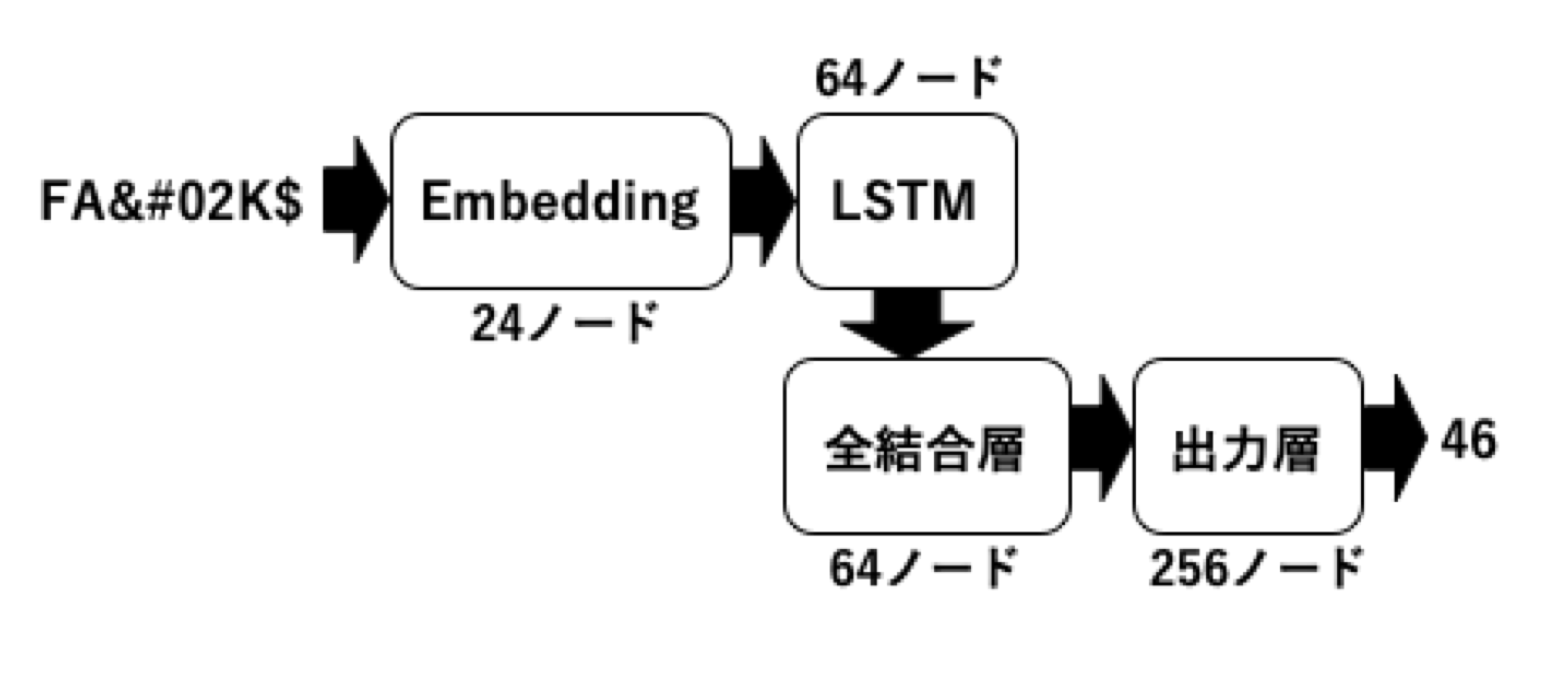
\includegraphics[width=100mm]{Namba_NN.eps}
\caption{難波\cite{namba}のニューラルネットワーク}
\label{namba}
\end{center}
\end{figure}

\begin{figure}[htbp]
\begin{center}
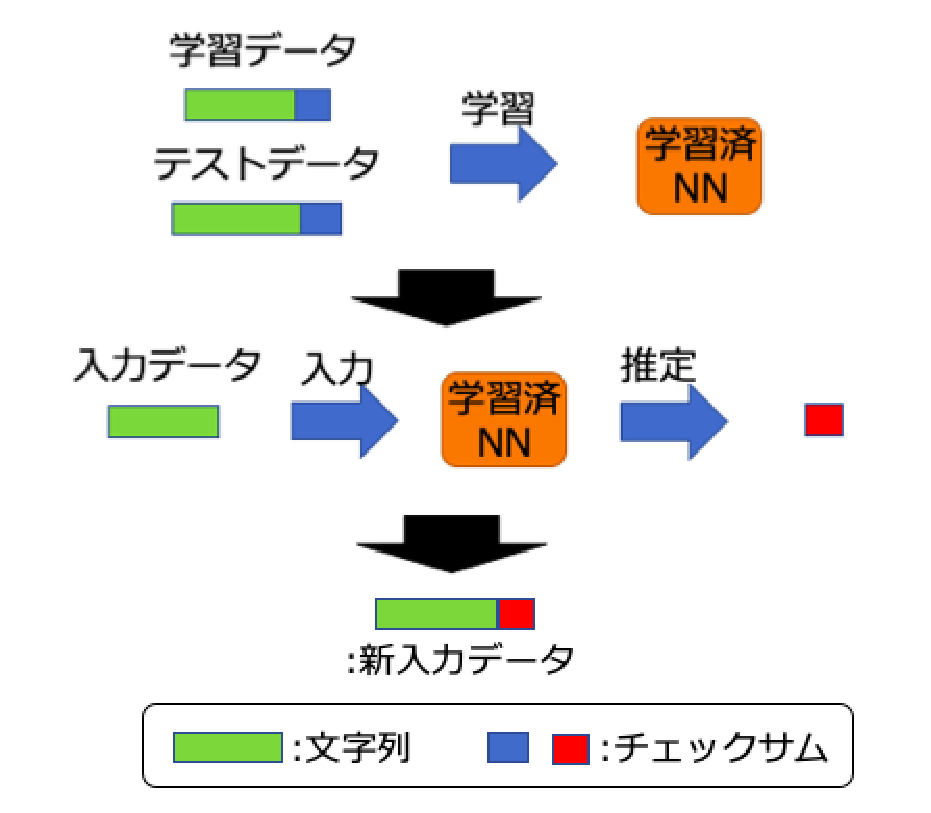
\includegraphics[width=100mm]{nambahantei.eps}
\caption{チェックサムの推定}
\label{hantei}
\end{center}
\end{figure}

\chapter{機械学習によるチェックサム及び \\ ハッシュ値の推定}

\section{可変長データに対応したニューラルネットワークによる学習}

本論文では, 難波\cite{namba}の汎用性を高めるため, 8 byte以上のデータに対するチェックサム及び様々なハッシュ値の推定を行う手法を提案する.
チェックサムおよびハッシュ値の学習には, 文字列とその文字列に対するチェックサムおよびハッシュ値のデータセットを使用する.
データとチェックサムおよびハッシュ値の位置とハッシュ関数の種類は既知であることを前提とする.
チェックサム及びハッシュ値の学習にはニューラルネットワークを使用して行う.

学習の仕組みを図\ref{suitei}に示す.
学習の仕組みは難波\cite{namba}と同様である.
難波\cite{namba}と異なる点として, チェックサム以外にCRC\cite{crc}, MD5\cite{md5}, SHA1\cite{sha1} のハッシュ値を推定する.
また, \cite{namba} byteの固定長の学習しか行なっていなかったため, 様々な長さの文字列である可変長データで学習を行う.

学習に使用するニューラルネットワークは, Encoder・Decoderモデル\cite{seq2seq}を利用したニューラルネットワークを構成して学習を行う.
また, ハッシュ関数によって計算方法は変わってくるため, 各々のハッシュ関数に対応した機械学習を行わなければならない.

可変長データの例を図\ref{kahen}に示す.
記号や数字, アルファベットの文字を1 byteとして扱う.
学習を行うデータとして, ランダム及び規則性のある文字列を扱う.

文字列の例を図\ref{fig:one}と図\ref{fig:two}に示す.
ランダム文字列は, 数字, 記号, アルファベットを乱雑に並べた文字列である.
この文字列を学習させることで, バイナリデータを変異ベース手法で入力データを作成するときに役立つ.
規則性のある文字列は, 日本語や英文など, 単語間に関係性をもつ文字列である.
この文字列を学習させることで, 主にテキストデータなどを変異ベース手法で入力データを作成するときに役立つ.

\begin{figure}[htbp]
\begin{center}
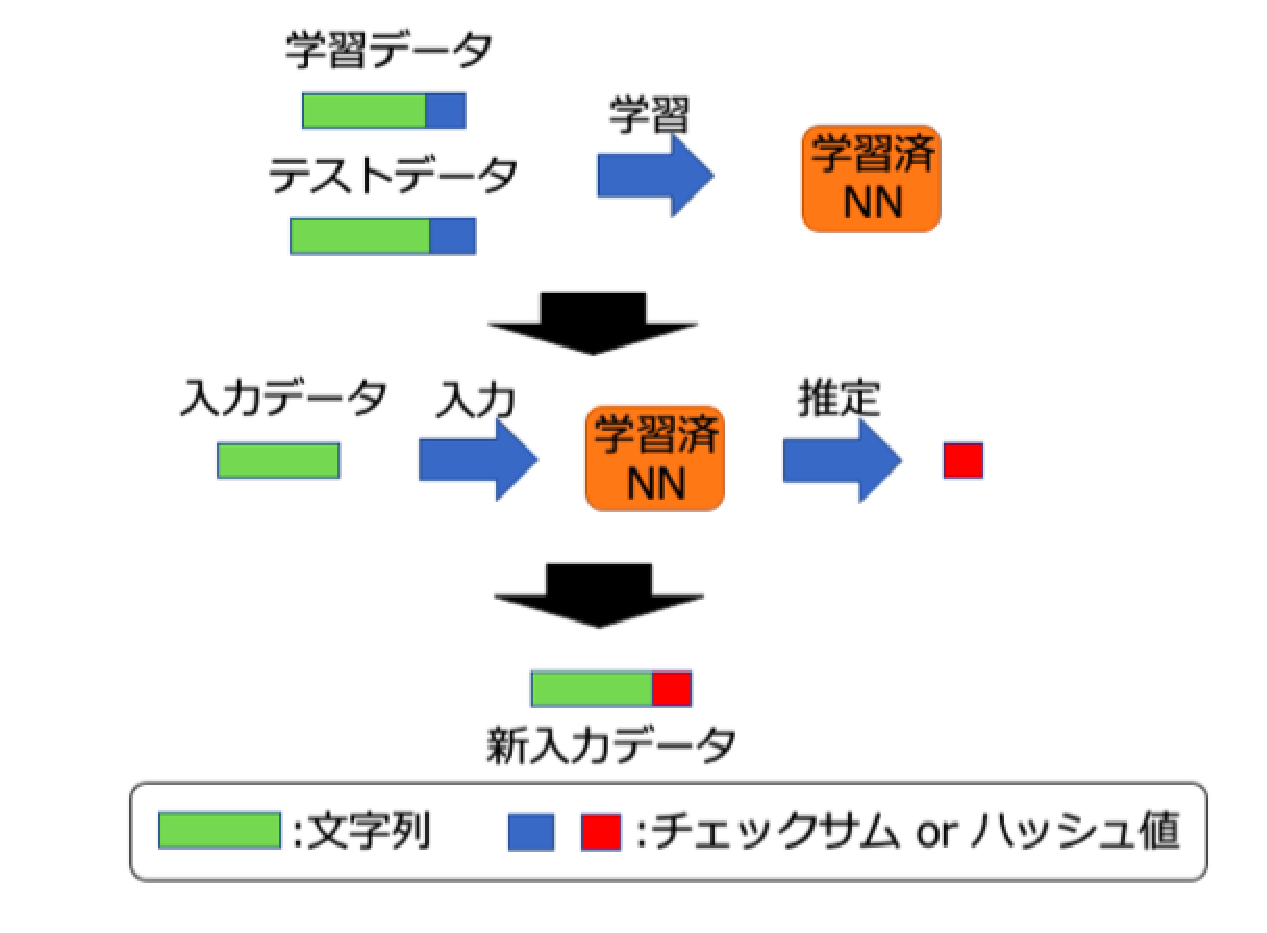
\includegraphics[width=130mm]{ataihantei.eps}
\caption{チェックサム及びハッシュ値の推定}
\label{suitei}
\end{center}
\end{figure}


\begin{figure}[htbp]
\begin{center}
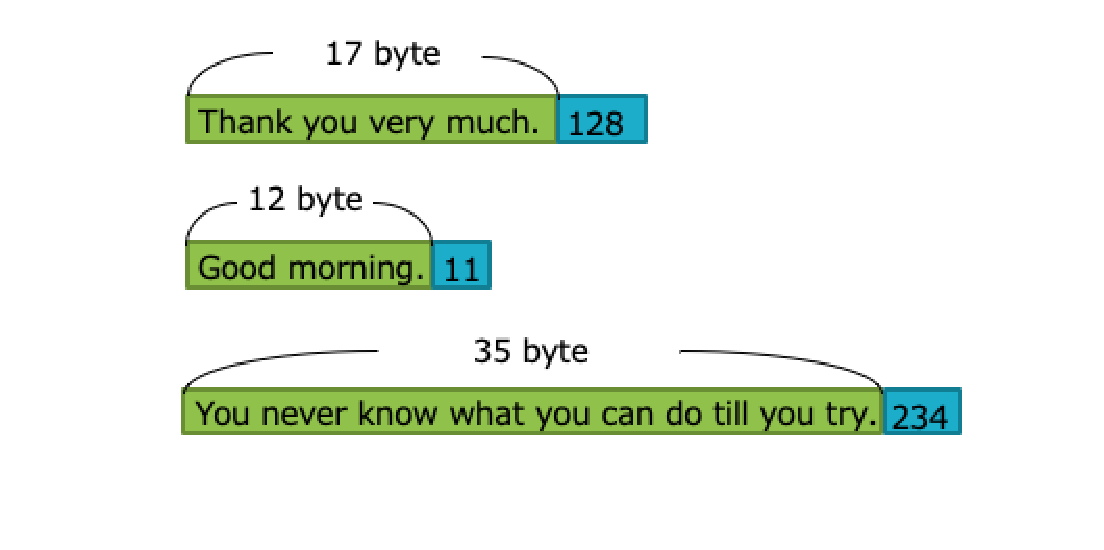
\includegraphics[width=120mm]{kahen.eps}
\caption{可変長データ}
\label{kahen}
\end{center}
\end{figure}


\begin{figure}[htbp]
 \begin{minipage}{0.5\hsize}
  \begin{center}
   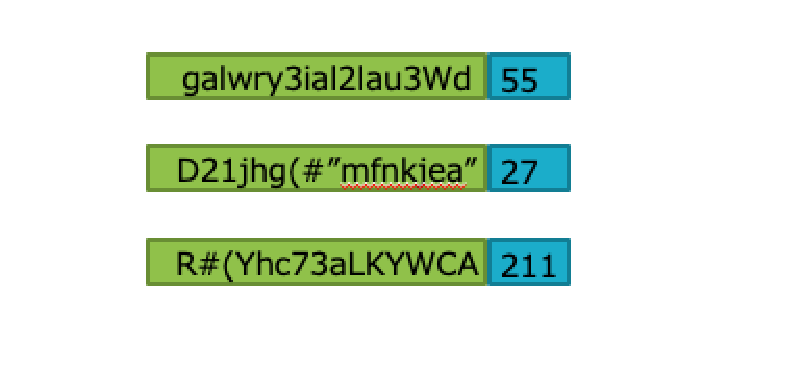
\includegraphics[width=100mm]{random.eps}
  \end{center}
  \caption{ランダム文字列}
  \label{fig:one}
 \end{minipage}
 \begin{minipage}{0.5\hsize}
  \begin{center}
   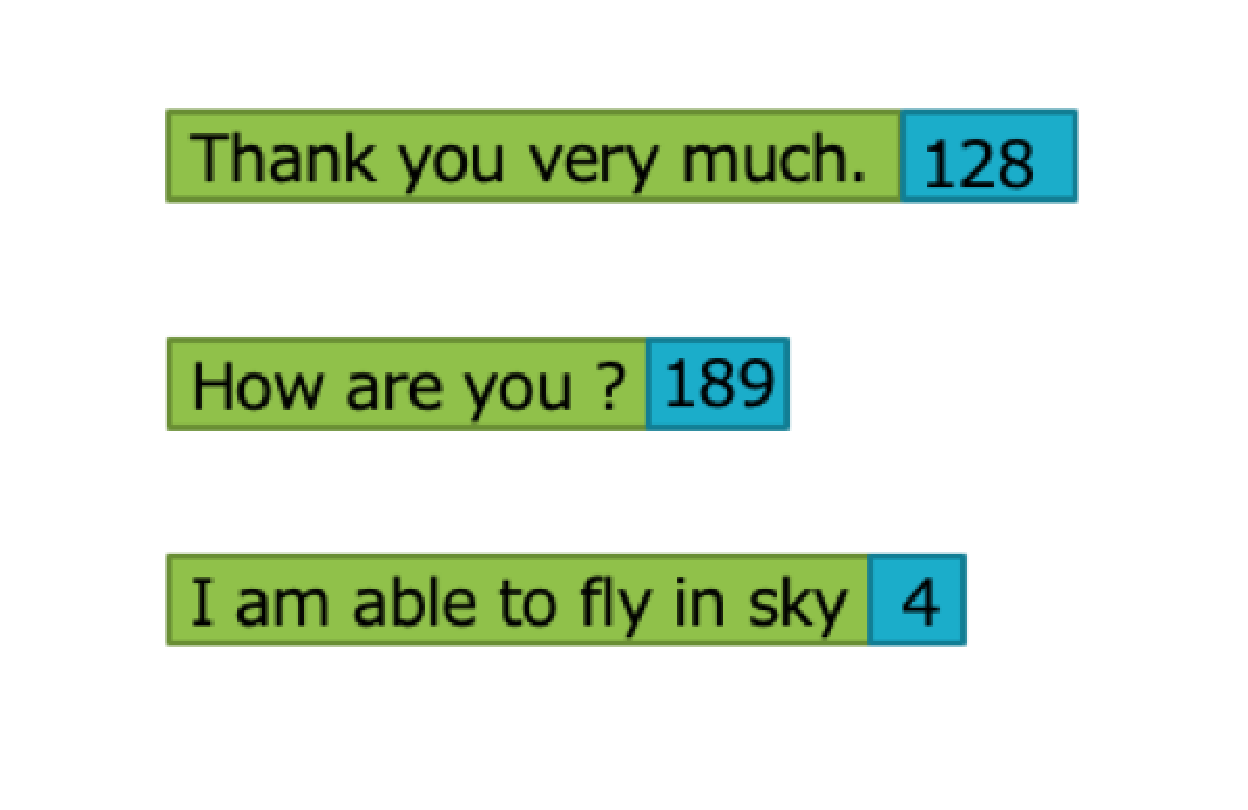
\includegraphics[width=70mm]{kisokusei.eps}
  \end{center}
  \caption{規則性のある文字列}
  \label{fig:two}
 \end{minipage}
\end{figure}

\newpage

\section{Encoder・Decoderモデルを用いた学習}
\subsection{Encoder・Decoderモデル}

Encoder・Decoderモデル\cite{namba}は自然言語処理系のニューラルネットワークである.
主に翻訳や文章の要約, 対話生成に使用される.

モデルの仕組みを図\ref{encdec}に示す.
この図は, 英語から日本語へと翻訳を行うニューラルネットワークである.
例として, Thank you very much.という文字列をEncoderへ入力する.

Encoderは画像,テキストなど何かしらの特徴ベクトルに変換する機構のことである.
入力した文字列に対して学習を行い, その処理した結果として内部状態を返す.
内部状態は, 入力データに対してベクトル化の処理を行った出力である.
ベクトル化を行った際, 各単語のベクトルの長さは全て一定にしなければならない.
次に, ベクトル化をした各単語の特徴ベクトルをDecoderへ入力する.

DecoderはEncoderでエンコードされた特徴ベクトルをデコードして何か新しいデータを生む機構のことである.
ターゲットとなる文字列の前の文字が与えられた場合, その次の文字を予測するように学習を行う.
学習を行う際, Decoderへの入力をEncoderへ入力した文字列の答えとなる文字列をあらかじめ用意する.
この時, 出力されるデータは, Encoderで入力したデータと同じデータ形式である必要はなく, 音声や動画など様々な形式で出力が可能である.

\subsection{ニューラルネットワークの構成}
ニューラルネットワークの構成は図\ref{model}を用いる.
Encoderにあたる箇所は, input\_1からlstm\_1までの層となる.
input\_1は文字列を入れる入力層である.
図の(None, None)はタプルであり, 主に層のノード数を表す.
各層のinputは, 層へ入力されるタプルで, outputは次の層へ出力するタプルである.
Noneの意味は, 任意の正の整数を意味する.
入力文字列の長さは一定ではないため, 入力層のノード数は各入力文字列の長さとなる.

embedding\_1はinput\_1から受け取った文字列のベクトル化を行う.
図のoutputの512がノード数であり, ベクトル化された文字の配列の長さとなる.

lstm\_1はembedding\_1から受け取った情報を元にLSTMによって計算を行う.
この時, 計算結果は破棄し, 計算過程などの内部状態のみを返す.

Decoderにあたる箇所は, input\_2からdense\_1までの層となる.
input\_2はEncoderへ入力した文字列に対する出力となる文字列を入れる入力層である.
input\_1と同様, ノード数は一定ではない.

embedding\_2はembedding\_1と同様にベクトル化を行い, lstm\_2で計算を行う.

lstm\_2では, lstm\_1と違い, 内部状態を破棄し, 計算結果を返す.
最終的に, lstm\_2で計算された結果をdense\_1の出力層で結果を出力する.
出力層のノード数が3 となっているのは, 出力する文字数が3 文字であることを意味する.

各ノード数などのパラメータは, どのような入力及び出力を行うかによって最適な値が異なるため, 何度も実験を繰り返して最適な値を見つける必要がある.
また, 全てのチェックサム及びハッシュ値を学習するにおいて, ニューラルネットワークの構成は同じである.

出力層は, 一般的なニューラルネットワークと違い, 出力される各文字に対して振り分けられる.
例として, 図\ref{output}にしめす.
Thank you!という文字列から180 となるチェックサムを推定するならば, 'Thank', 'you', '!'の3 つの単語に分割し, 入力をし学習を行う.
推定を行う際に, 初めの1 文字目が1 $\sim$ 9 または空白なのかを1/10 で予測し, 出力する.
それを最後の文字まで続け, その結果の予測値と真理値が同じになるように重みを更新していく.
I don't think so. という文字列の推定結果の1 文字目の$\textless$ $\textgreater$は空白を表す.
この空白は, 1 文字として扱う.
3 つ目のI am fine. からCRC16 を推定するならば, 0 と1 及び空白の1/3 で各文字を予測する.



\begin{figure}[htbp]
\begin{center}
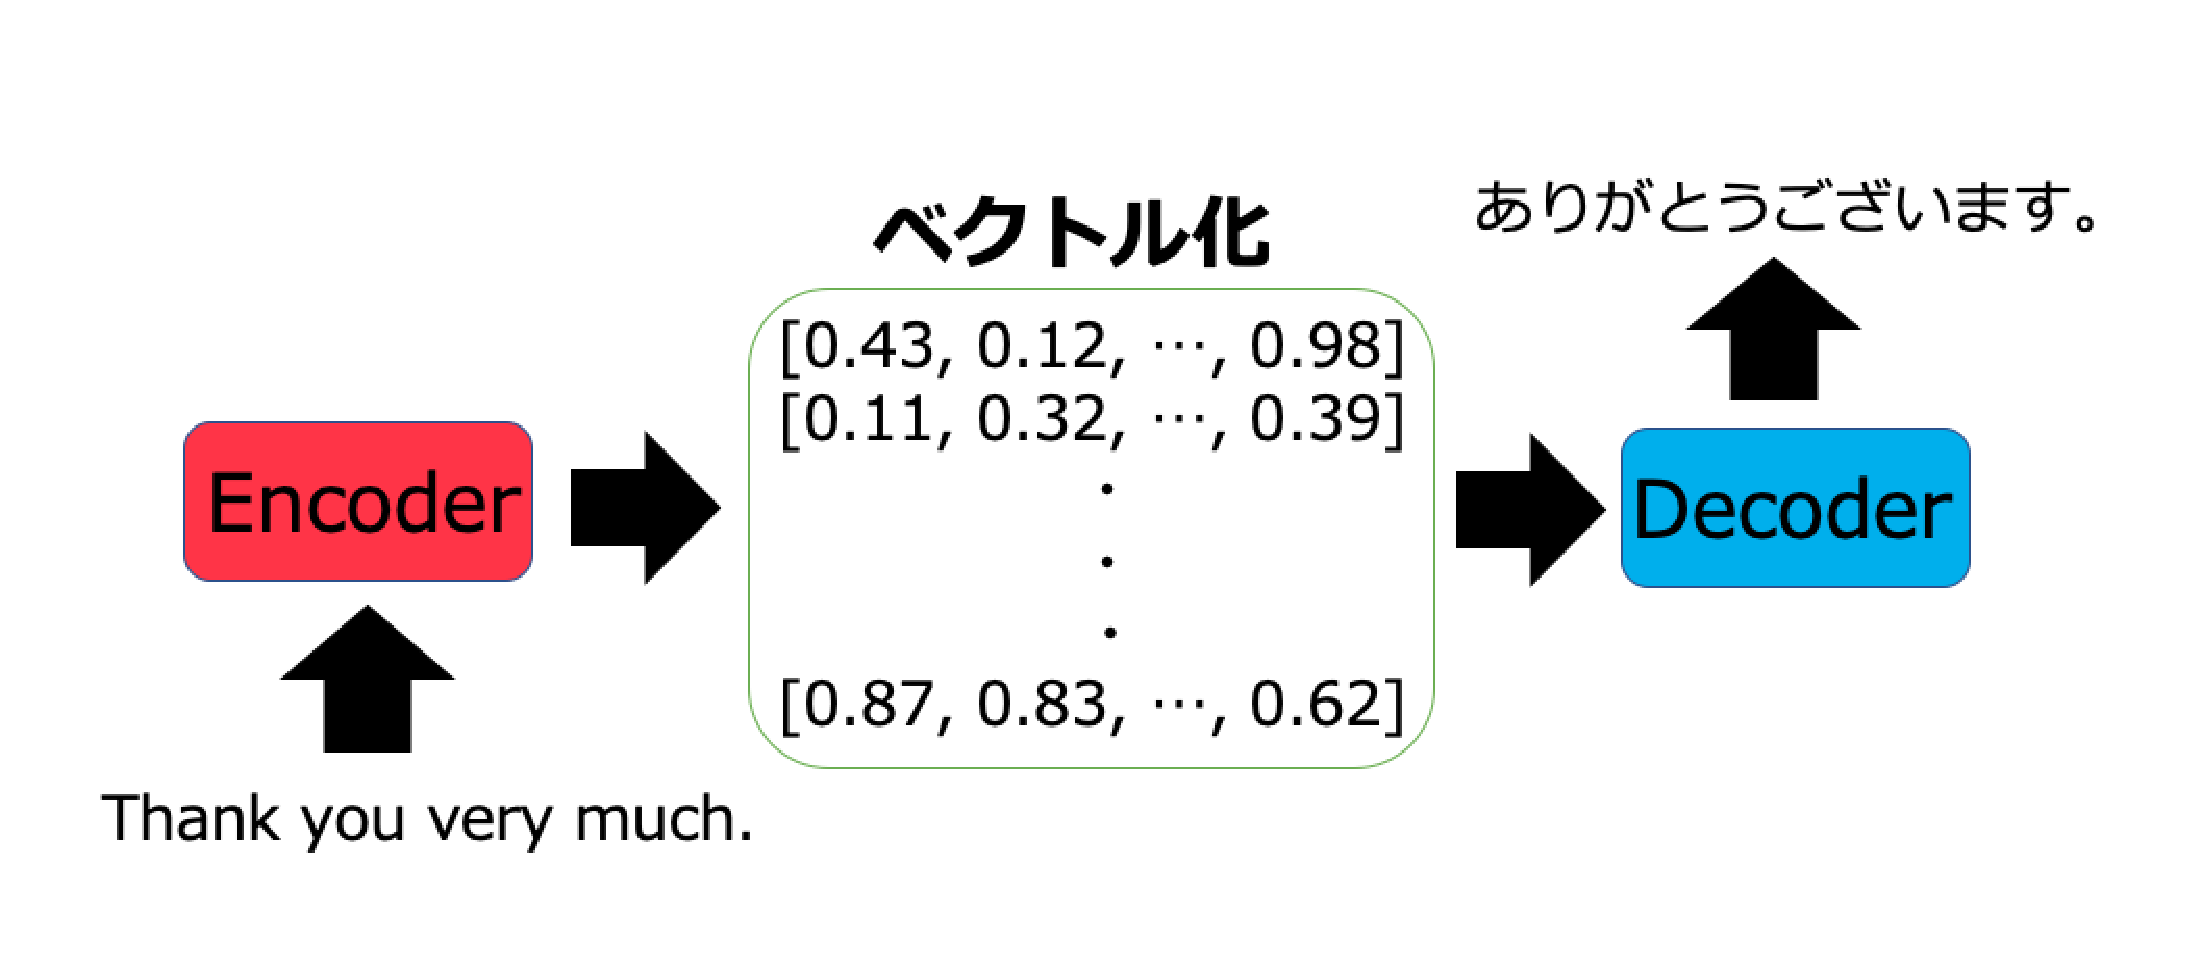
\includegraphics[width=150mm]{encdec.eps}
\caption{Encoder・Decoderモデル}
\label{encdec}
\end{center}
\end{figure}

\begin{figure}[htbp]
\begin{center}
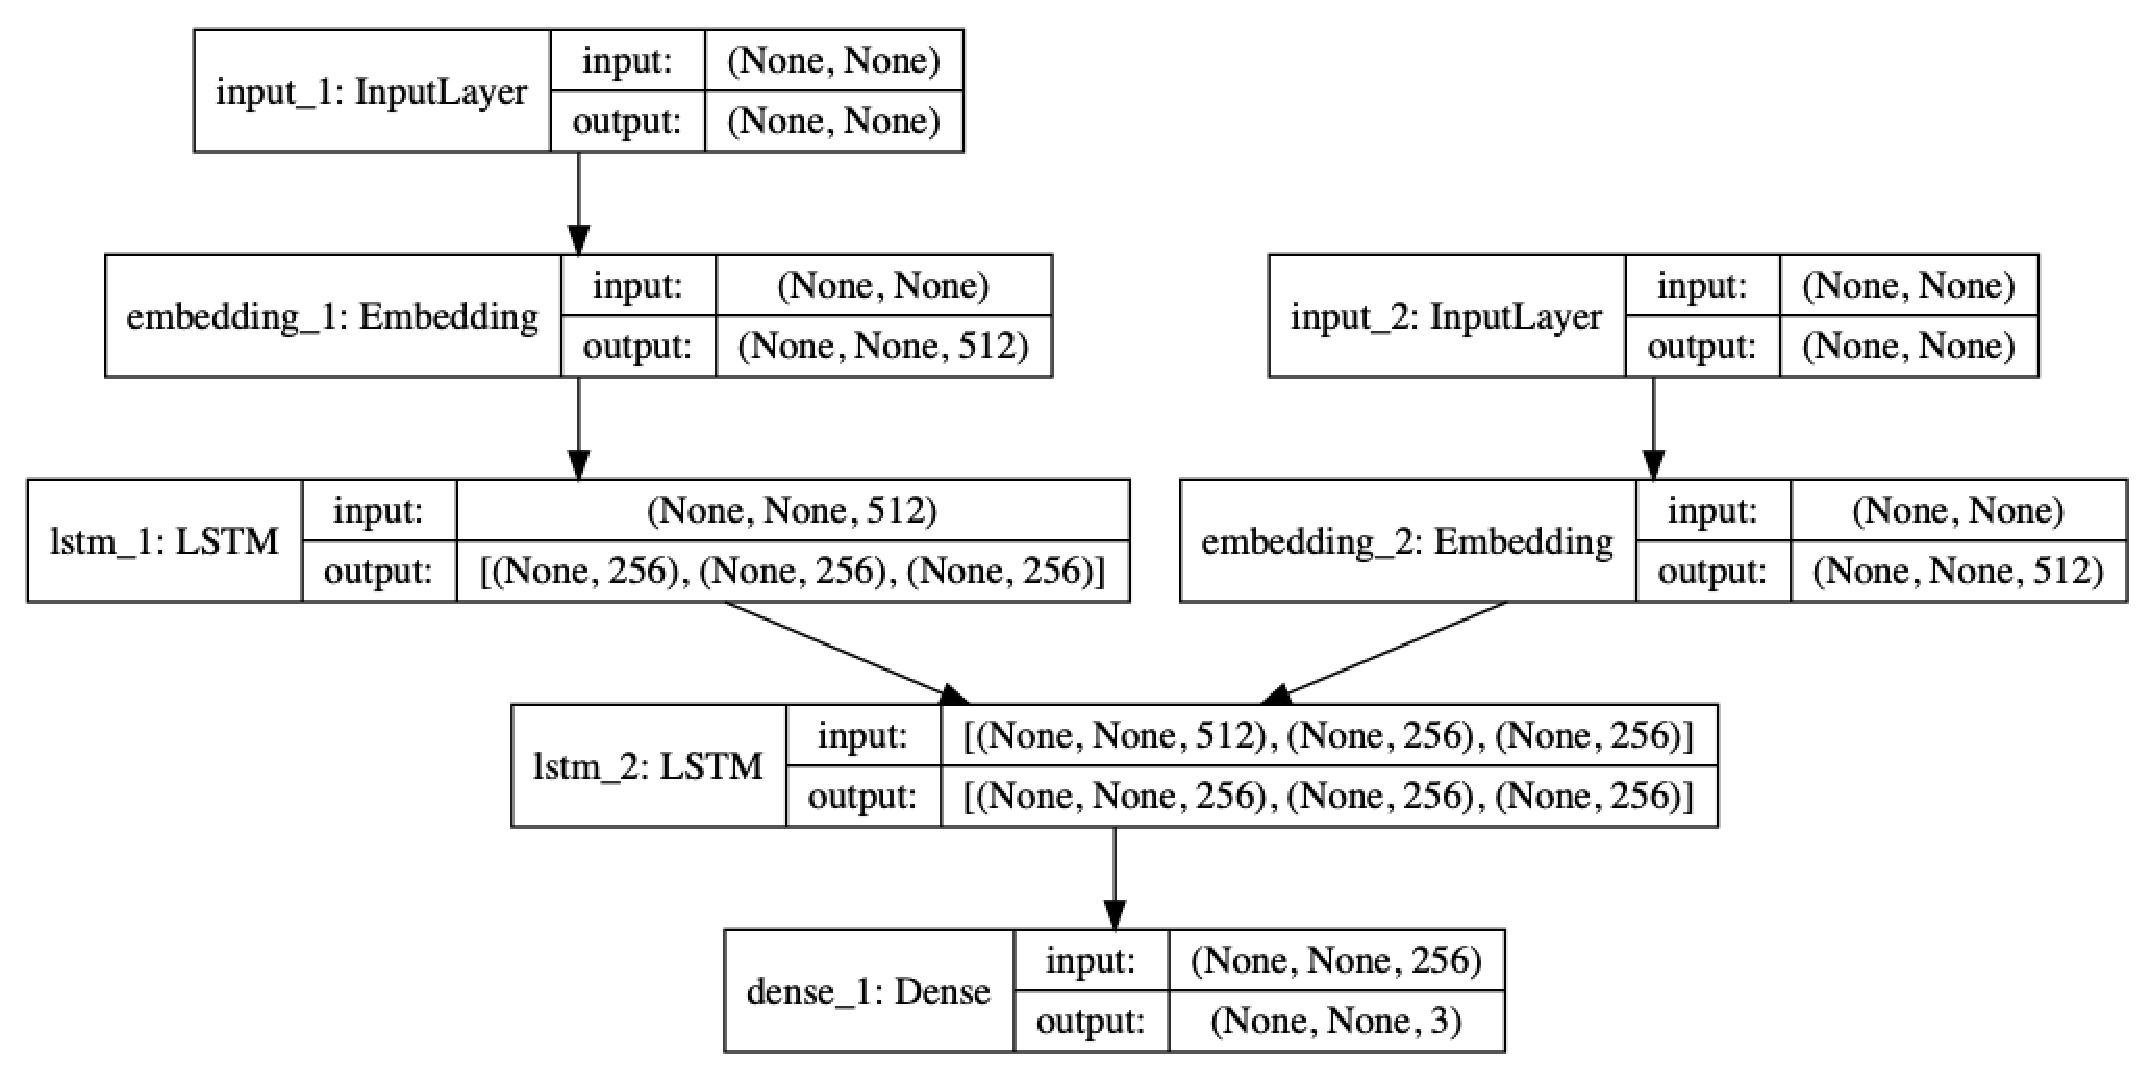
\includegraphics[width=150mm]{NN_model.eps}
\caption{ニューラルネットワーク}
\label{model}
\end{center}
\end{figure}

\begin{figure}[htbp]
\begin{center}
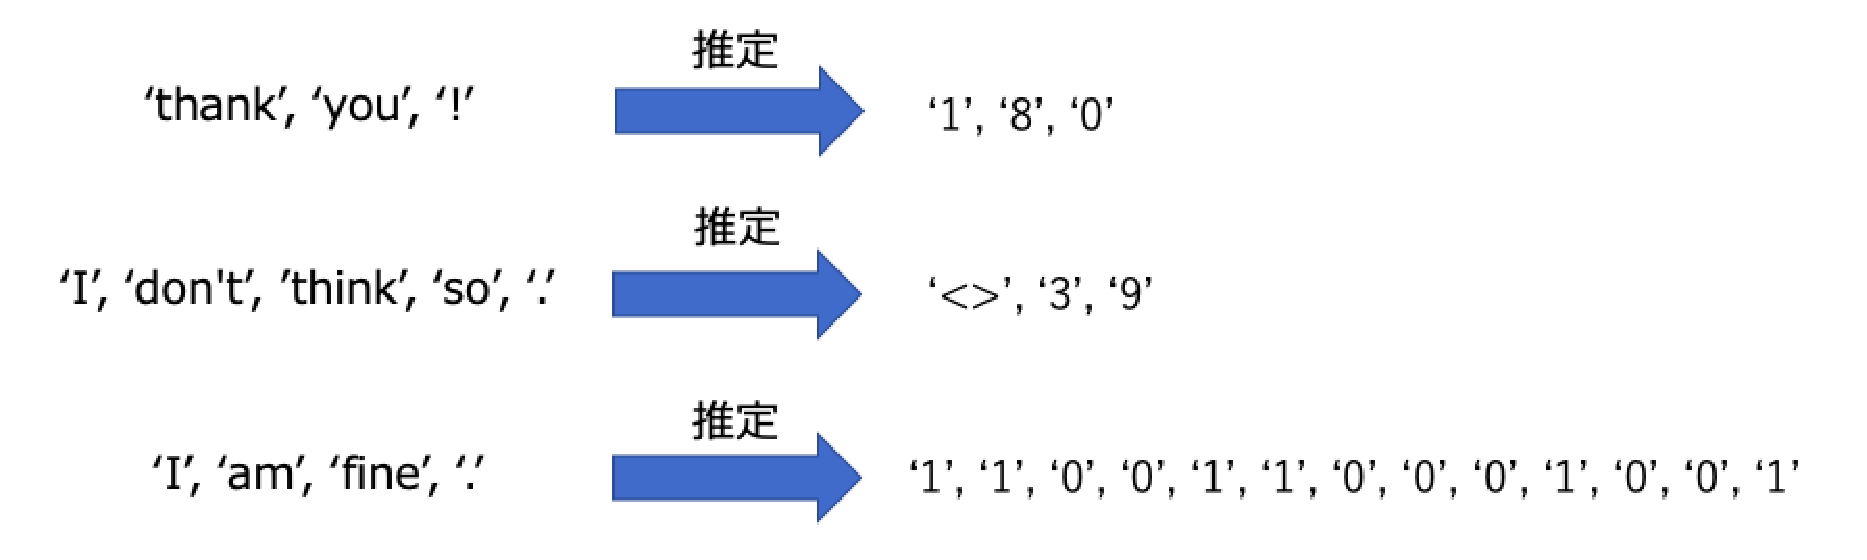
\includegraphics[width=150mm]{output.eps}
\caption{出力の構成}
\label{output}
\end{center}
\end{figure}


\chapter{実装と実験結果}
\section{実装}

本研究では, 機械学習を用いて8 byte以上のランダム文字列と規則性のある文字列に対するチェックサム及びハッシュ値の推定を行った.
データセットは, Perlにある文字列からチェックサム及びハッシュ値を計算するモジュールを使用して作成した.
文字列には, ランダム文字列と規則性のある文字列として英文を起用した.
提案手法をKerasを用いてPythonで実装し, 機械学習を実行した.
文字列とチェックサム及びハッシュ値のデータセットは, 各学習に置いて最適なデータ数を用意した.
ハッシュ関数はCRC16\cite{crc}, CRC32\cite{crc}, MD5\cite{md5}, SHA1\cite{sha1} を使用した.
学習に用いたニューラルネットワークは, Encoder・Decoderモデルを使用した.
学習回数はチェックサム及びハッシュ値によって異なる.
オプティマイザにはAdamを使用した.


\section{実験}

機械学習を用いてランダム文字列と規則性のある文字列に対するチェックサム及びハッシュ値を推定する実験を行った.
学習の仕組みを図\ref{gakusyu}に示す.
初めに, 文字列と文字列に対するチェックサム及びハッシュ値の2 種類のデータを用意する.
次に, そのデータを教師データとテストデータに分割する.
教師データは, ニューラルネットワークに学習させるためのデータであり, テストデータは, 実際に学習ができているのか確認するためのデータである.
そして, 教師データを使って学習を行う.
教師データ全てを使って一度学習を終えたのちに, テストデータで確認を行う.
ニューラルネットワークが予測した値と正解の値を比較し, 間違っていれば, その乖離をなくすために再度学習を行う.
この時, 汎化性能を高めるために, 学習精度は教師データで学ばせた時より, テストデータで確認を行った時の方が高いように学習を行わなければならない.


\begin{figure}[htbp]
\begin{center}
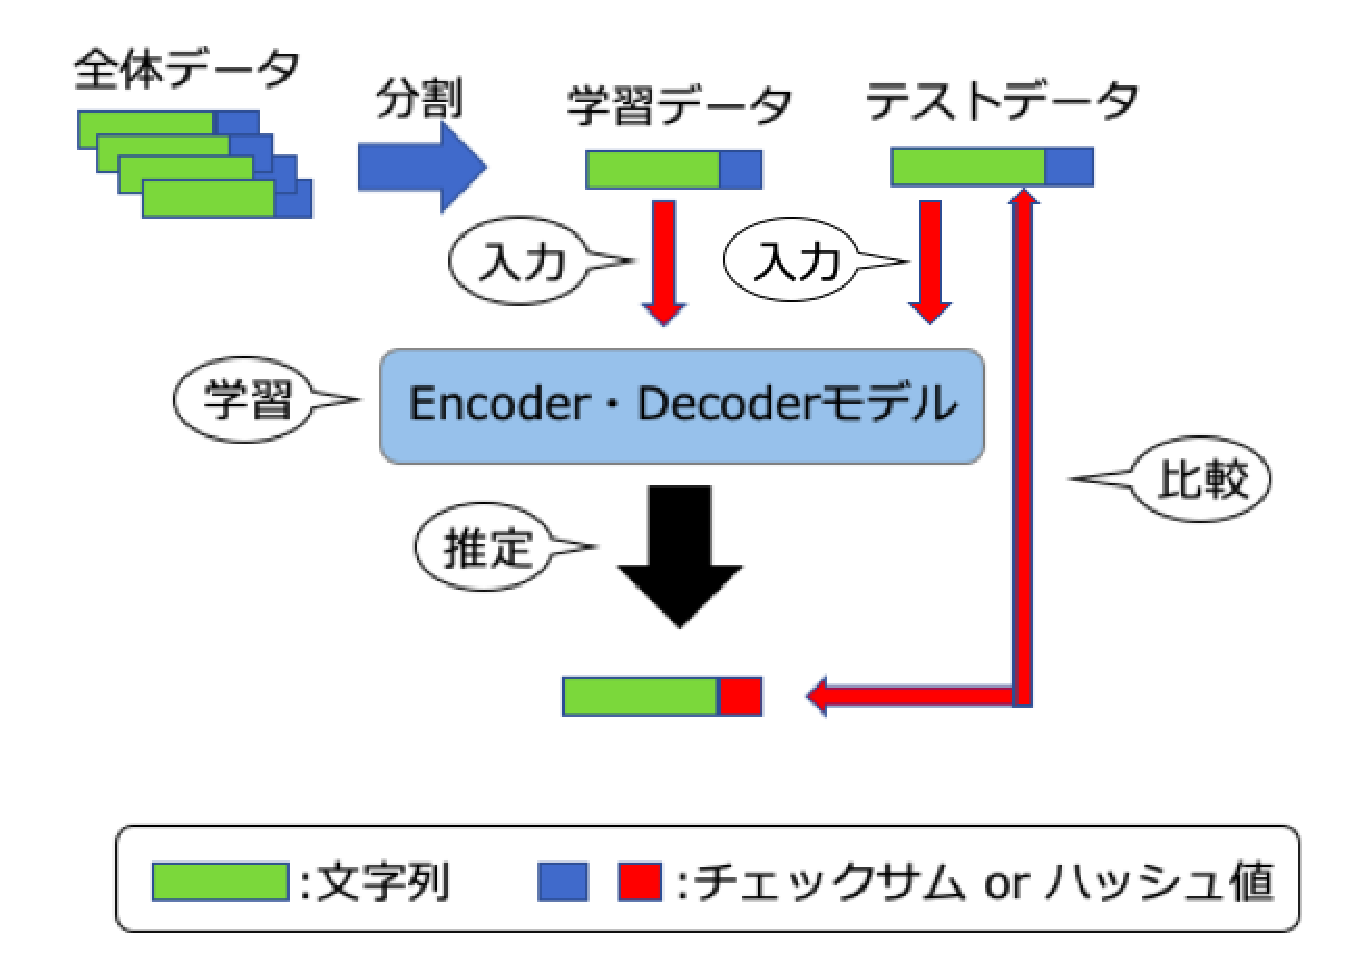
\includegraphics[width=130mm]{hantei.eps}
\caption{学習の流れ}
\label{gakusyu}
\end{center}
\end{figure}

\newpage

\section{学習結果}

英文の学習結果を, 表\ref{english}に示す.
文字列は可変長の入力データである.
train data とtest dataは, 学習データとテストデータで学習を行った時の学習精度を表す.
train loss 及びtest loss は, 学習及び推定した結果と実際の正解と比較して, どれほどの乖離があったのか表す.
byte は, 学習を行った文字列のbyte数を表す.
epoch は, 学習を行った回数を表す.
lstm nodeは, LSTM のノード数を表す.

全体のテストデータの結果から, チェックサムと各ハッシュにおいて, 学習をしていない状態より遥かに高い精度が得られた.
また, 学習データとテストデータがほぼ同じ精度となっているため, 理想的な機械学習をしていると考えられる.
しかし, MD5とSHA1の損失値が高い傾向にあるため, 学習方法を改善しなければならない.

ランダム文字列の学習結果を, 表\ref{random}に示す.
文字列は可変長の入力データである.
train data とtest data は, 各データで学習を行った時の学習精度を表す.
train loss 及びtest lossは, 学習及び推定した結果と実際の正解と比較して, どれほどの乖離があったのか表す.
表のbyte という項目は, 学習を行った文字列のbyte数を表す.
epoch は, 学習を行った回数を表す.

規則性のある文字列と比較を行うと, 全体的に精度が低い傾向となっている.
また, 学習誤差, 推定誤差も高い傾向にある.
原因として, 文字列に関係性がないため, そこから正解を予測するための基準を理解させるのが困難であると考えられる.


\begin{table}[htp]
   \begin{center}
    \caption{英文の学習精度}
    \small
    \smallskip
    \begin{tabular}{|l|r|r|r|r|r|r|r|r|}
    \hline
      &\texttt{train data }&\texttt{test data }&\texttt{train loss }&\texttt{test loss  }&\texttt{byte }&\texttt{epoch }&\texttt{data} & \texttt{lstm node} \\ \hline
    \texttt{checksum  }&\texttt{50\% }&\texttt{50\% }&\texttt{0.27  }&\texttt{0.24 }&\texttt{2 $\sim$ 48 }&\texttt{100 }&\texttt{12 万 }&\texttt{64} \\ \hline
    \texttt{CRC16  }&\texttt{47\% }&\texttt{47\% }&\texttt{0.57 }&\texttt{0.57  }&\texttt{2 $\sim$ 16 }&\texttt{120 }&\texttt{12 万 }&\texttt{64 } \\ \hline
    \texttt{CRC32  }&\texttt{49\% }&\texttt{50\% }&\texttt{0.59 }&\texttt{0.59  }&\texttt{2 $\sim$ 18 }&\texttt{100 }&\texttt{10 万 }&\texttt{48}\\ \hline
    \texttt{MD5 }&\texttt{11\% }&\texttt{11\% }&\texttt{2.45  }&\texttt{2.45  }&\texttt{2 $\sim$ 19 }&\texttt{100 }&\texttt{20 万 }&\texttt{128} \\ \hline
    \texttt{SHA1    }&\texttt{19\% }&\texttt{19\% }&\texttt{2.2  }&\texttt{2.2  }&\texttt{2 $\sim$ 18 }&\texttt{100 }&\texttt{12 万 }&\texttt{256}\\ \hline

    \end{tabular}
    \label{english}
   \end{center}

\end{table}

\begin{table}[htp]
   \begin{center}
    \caption{ランダム文字列の学習精度}
    \small
    \smallskip
    \begin{tabular}{|l|r|r|r|r|r|r|r|r|}
    \hline
       &\texttt{train data }&\texttt{test data }&\texttt{train loss }&\texttt{test loss  }&\texttt{byte }&\texttt{epoch }&\texttt{data }& \texttt{lstm node} \\ \hline
    \texttt{checksum   }&\texttt{51\% }&\texttt{52\% }&\texttt{0.48 }&\texttt{0.48 }&\texttt{1 $\sim$ 32 }&\texttt{300 }&\texttt{10 万 }&\texttt{64}\\ \hline
    \texttt{CRC16   }&\texttt{53\% }&\texttt{53\% }&\texttt{0.53 }&\texttt{0.53 }&\texttt{1 $\sim$ 16 }&\texttt{130 }&\texttt{16 万 }&\texttt{32}\\ \hline
    \texttt{CRC32   }&\texttt{54\% }&\texttt{54\% }&\texttt{0.57 }&\texttt{0.57 }&\texttt{1 $\sim$ 8 }&\texttt{100 }&\texttt{10 万 }&\texttt{52}\\ \hline
    \texttt{MD5  }&\texttt{11\% }&\texttt{11\% }&\texttt{2.27  }&\texttt{2.22  }&\texttt{1 $\sim$ 8 }&\texttt{100 }&\texttt{20 万 }&\texttt{128}\\ \hline
    \texttt{SHA1    }&\texttt{14\% }&\texttt{14\% }&\texttt{2.47  }&\texttt{2.47  }&\texttt{1 $\sim$ 8 }&\texttt{50 }&\texttt{20 万 }&\texttt{128}\\ \hline
    \end{tabular}
    \label{random}
   \end{center}

\end{table}


\section{学習結果の検証}

表\ref{english}と表\ref{random}に示した結果は期待以上の成果であったが, これらの学習精度は目安としかならない.
一般的なニューラルネットワークの場合, 学習精度はニューラルネットワークが予測した結果と実際の正解と完全に一致した数から, 検査したデータ数の割合から出力される.
このEncoder・Decoderモデル\cite{seq2seq}は, 出力した結果の1 文字ずつに対して判定を行う.
つまり, 予測した結果と実際の正解が完全に一致しなくても, 正解の文字が1 つでも含まれていれば良い.
そのため, 実際に推定を行う際と異なる正答率である可能性が高いことがわかる.

本来の学習精度を測るために, 学習済ニューラルネットワークを使って, 文字列からチェックサム及びハッシュ値の推定を行った.
ランダム文字列及び英文の正答率を表\ref{seitouritu}に示す.
random, englishが学習済ニューラルネットワークを使用した時に得られた正答率である.
train random, train englishは, 学習時に得られた正答率である.
検証に使用したデータは, 学習時に使用したテストデータにある1 万個の文書を用いて行なった.

学習時に得られた正答率と学習済ニューラルネットワークを使用して得られた正答率を比較すると, 必ずしも正答率が一致しないことがわかった.
特に, チェックサムまたはハッシュ値によって, ランダム文字列の方が正答率が高かったり, 英文の方が正答率が高かったりなど, ばらつきが見られた.
原因として, 適切なLSTMのノード数を設定出来ていなかったり, データセットが不十分であったりなど考えられる.
また, ニューラルネットワークの構成自体が適切でない可能性もあるため, 更なる実験及び検証が必要である.

\begin{table}[htp]
   \begin{center}
    \caption{学習済ニューラルネットワークを用いたチェックサム及びハッシュ値の推定}
    \smallskip
    \begin{tabular}{|l|r|r|r|r|}
    \hline
       &\texttt{random  }&\texttt{english  }&\texttt{train random }&\texttt{train english} \\ \hline
    \texttt{checksum   }&\texttt{20\% }&\texttt{50.8\%  }&\texttt{52\% }&\texttt{50\% }\\ \hline
    \texttt{CRC16     }&\texttt{9.01\% }&\texttt{9.08\% }&\texttt{53\% }&\texttt{47\%   } \\ \hline
    \texttt{CRC32    }&\texttt{11.9\% }&\texttt{4.17\%  }&\texttt{54\% }&\texttt{50\%  }  \\ \hline
    \texttt{MD5   }&\texttt{12.07\% }&\texttt{2.53\%  }&\texttt{11\% }&\texttt{11\%   } \\ \hline
    \texttt{SHA1    }&\texttt{4.95\% }&\texttt{10.75\%  }&\texttt{14\% }&\texttt{19\%}    \\ \hline
    \end{tabular}
    \label{seitouritu}
   \end{center}

\end{table}

\newpage

1 $\sim$ 32 byteのランダム文字列と2 $\sim$ 48 byteの英文に対するチェックサムの推定結果の一部を表\ref{cksum_suitei}に示す.
Inputが入力文字列であり, Decodeが推定結果, Accuracyが入力文字列に対する正解の出力である.\\


\begin{table}[htp]
   \begin{center}
    \caption{チェックサムの推定}
    \smallskip
    \begin{tabular}{|l|r|r|r|}
    \hline
       &\texttt{Input }&\texttt{Decode }&\texttt{Accuracy}   \\ \hline
     &\texttt{6duf]LiT\}`KE:UCJ }&\texttt{110 }&\texttt{100} \\ \cline{2-4}
    \texttt{Random }&\texttt{773=d\#E4k\%1UF2q }&\texttt{0 }&\texttt{0} \\ \cline{2-4}
    &\texttt{ 8H?v;+6 }&\texttt{208 }&\texttt{209}  \\ \hline
    &\texttt{may i profess my love?  }&\texttt{14 }&\texttt{13} \\ \cline{2-4}
   \texttt{English }&\texttt{i'm telling you that... }&\texttt{208 }&\texttt{208} \\ \cline{2-4}
   &\texttt{ get him down. }&\texttt{165 }&\texttt{164 } \\ \hline

    \end{tabular}
    \label{cksum_suitei}
   \end{center}

\end{table}


推定結果から, 不正解だった推定結果と正解を比較すると, 正解から1 $\sim$ 10の誤差で値を出力していることがわかった.
原因は調査中であるが, 一部の文字列に対して計算を行っていない可能性がある.
この原因を解決することが出来れば, 更なる精度向上が見込まれる.
ランダム文字列の結果と比較すると, 英文などの規則性のある文字列の方が高い精度が得られることがわかる.
原因として, 規則性のある文字列の方が, 文字列の関係性がはっきりしているため, 計算アルゴリズムが理解しやすいと考えられる.

\newpage

1 $\sim$ 16 byteのランダム文字列と2 $\sim$ 16 byteの英文に対するCRC16 の推定結果の一部を表\ref{crc16_suitei}に,
1 $\sim$ 8 byteのランダム文字列と2 $\sim$ 18 byteの英文に対するCRC32 の推定結果の一部を表\ref{crc32_suitei}に, 示す.
Inputが入力文字列であり, Decodeが推定結果, Accuracyが入力文字列に対する正解の出力である.\\

\begin{table}[htp]
   \begin{center}
    \caption{CRC16 の推定}
    \smallskip
    \begin{tabular}{|l|l|r|r|}
    \hline
       &\texttt{Input }&\texttt{Decode }&\texttt{Accuracy}   \\ \hline
     &\texttt{b\%.H]|[0@B\*!\^dP }&\texttt{110101010101 }&\texttt{101010101110} \\ \cline{2-4}
    \texttt{Random }&\texttt{EER9V\{Ta }&\texttt{11100101 }&\texttt{11100101} \\ \cline{2-4}
    &\texttt{ w\/YAQCklLUX5fW }&\texttt{110101010110 }&\texttt{101010101010}  \\ \hline
    &\texttt{i do.  }&\texttt{1111101010111011 }&\texttt{1111101010111011} \\ \cline{2-4}
   \texttt{English }&\texttt{just do it. }&\texttt{1010100010100101 }&\texttt{10100000111011} \\ \cline{2-4}
   &\texttt{ so i was happy. }&\texttt{1011011111110101 }&\texttt{101000101101001}  \\ \hline

    \end{tabular}
    \label{crc16_suitei}
   \end{center}

\end{table}

\begin{table}[htp]
   \begin{center}
    \caption{CRC32 の推定}
    \small
    \smallskip
        \scalebox{0.8}{
    \begin{tabular}{|l|l|r|r|}
    \hline
       &\texttt{Input }&\texttt{Decode }&\texttt{Accuracy}   \\ \hline
     &\texttt{muah }&\texttt{0010101001110011000000111111101 }&\texttt{1001000011101001010001101101} \\ \cline{2-4}
    \texttt{Random }&\texttt{o }&\texttt{1111000011111001001101000100 }&\texttt{1111000011111001001101000100} \\ \cline{2-4}
    &\texttt{ =!\#U\<\^  }&\texttt{1110010111110011100011110011010 }&\texttt{11010010010101110101101011100011}  \\ \hline
    &\texttt{storm!  }&\texttt{10011000001011001100011000011100 }&\texttt{10011000001011001100011000011100} \\ \cline{2-4}
   \texttt{English }&\texttt{stop! listen! }&\texttt{11111100001111111100010111111111 }&\texttt{10110110010101100111010111111000} \\ \cline{2-4}
   &\texttt{ who's a killer? }&\texttt{1111010000111111100010000001111 }&\texttt{1000100110110000001000100111001}  \\ \hline

    \end{tabular}
    }
    \label{crc32_suitei}
   \end{center}

\end{table}

CRC16 の推定結果から, 正解に近い値を出力していることが多く, 完全に答えと一致しているものは少ないことがわかった.
また, 正解と推定結果のbit数が殆ど一致しているのが見受けられた.
英文と比較して, ランダム文字列と同様, 不正解だった出力でも正解と近い出力をしていることがわかった.
しかし, より長い文字列の場合, 殆ど推定が出来ていなかった.

CRC32 の推定結果から, CRC16 と同様に, 正解に近い値を出力しているが, 完全に答えと一致している値は少なかった.
また, 出力が全て固定長でなく, 様々な組み合わせの出力がされていることが見受けられるため, 学習が全くできていないという可能性は低いことがわかった.
しかし, 正解と同じ値が出力された文字列の多くが1 または2 byteの時だった.
学習精度からCRC16 と比較して, CRC32 の方が正確に出力していることがわかった.
出力が短い方が推定するのが容易であると考えていたが, 恐らく学習させた文字列の長さの違いによるものである可能性が高い.

\newpage

1 $\sim$ 8 byteのランダム文字列と2 $\sim$ 19 byteの英文に対するMD5 の推定結果の一部を表\ref{md5_suitei}に示す.
Inputが入力文字列であり, Decodeが推定結果, Accuracyが入力文字列に対する正解の出力である.\\

\begin{table}[htp]

    \caption{MD5 の推定}
    \smallskip
    \small
    \begin{tabular}{|l|l|r|r|}
    \hline
       &\texttt{Input }&\texttt{Decode }&\texttt{Accuracy}    \\ \hline
     &\texttt{POB3\}-\{g }&\texttt{b7bc8c67d658878888888946646664b6 }&\texttt{400577e173ace391fc109e78f737d58d} \\ \cline{2-4}
    \texttt{Random }&\texttt{y:n\}W,/S}&\texttt{5dc4d646666666666888888888883877 }&\texttt{b2d6d53f53a22a4117c97f92da16bfda} \\ \cline{2-4}
    &\texttt{ H }&\texttt{c1d9f50f86825a1a2302ec2449c17196 }&\texttt{c1d9f50f86825a1a2302ec2449c17196}  \\ \hline
    &\texttt{what!?  }&\texttt{7ee3f61af1b2b7f3f1607aac1cc86f8c }&\texttt{7ee3f61af1b2b7f3f1607aac1cc86f8c} \\ \cline{2-4}
   \texttt{English }&\texttt{it is? }&\texttt{95fa3ec416cbdf2adf2a6ae4bca3435f }&\texttt{95fa3ec416cbdf2adf2a6ae4bca3435f} \\ \cline{2-4}
   &\texttt{  mumbler! }&\texttt{b040dd95a762d45aab4f4f54f4f33592 }&\texttt{3b7642c8f4a0a25539dff4aaeb0509cf} \\ \hline

    \end{tabular}
    \label{md5_suitei}

\end{table}

ランダム文字列は, どの入力文字列に対しても, 同じような出力をしていることがわかる.
特定の文字や文字列の長さに関わらず出力しているため, 原因はわからなかった.
また, 実際に推定ができた文字列は, 入力文字列が1 byteのみであった,
このことから, MD5 のアルゴリズムをニューラルネットワークで理解させるのは非常に困難であることがわかった.
英文は, 6 byte以下の文字列であれば, 正解又は正解に近い値を出力することがわかった.
これより, ランダム文字列より的確に推定結果を出力出来ていることがわかった.
ランダム文字列の方が正答率は高いが, 正解を出力することができる文字列は英文の方が高かった.
%1 万個の文字列のうち, 253 個正解だったため, 学習精度は約2.53\%である.
%実際にランダムでMD5 を当てる確率は2.93874E-39\%であるため, 比較するとこの学習精度は約1.07087E+40 倍高いと言える.

1 $\sim$ 8 byteのランダム文字列と2 $\sim$ 18 byteの英文に対するSHA1 の推定結果の一部を表\ref{sha1_suitei}に示す.
Inputが入力文字列であり, Decodeが推定結果, Accuracyが入力文字列に対する正解の出力である.\\

\begin{table}[htp]
   \begin{center}
    \caption{SHA1 の推定}
    \small
    \scalebox{0.8}{
    \begin{tabular}{|l|l|r|r|}
    \hline
      &\texttt{Input }&\texttt{Decode }&\texttt{Accuracy}    \\ \hline
     &\texttt{ ( }& \texttt{28ed3a797da3c48c309a4ef792147f3c56cfec40 } & \texttt{28ed3a797da3c48c309a4ef792147f3c56cfec40} \\ \cline{2-4}
    \texttt{Random }& \texttt{pz }& \texttt{e0fd60007dd0003a70071010701060606d64bbbb536 }& \texttt{5ffaa7bd95eb19342dcbb20cc58fc75e712c5847} \\ \cline{2-4}
    & \texttt{ vndf3 }& \texttt{1000710003a64607070707011d007070707070fc6fc } &\texttt{2fcc715443472d5bc62bde7300e7ff7d8698edff}  \\ \hline
    & \texttt{i see.  } &\texttt{bf39d91277ed1c47df88ed5771ef8134ceddac75 } &\texttt{bf39d91277ed1c47df88ed5771ef8134ceddac75} \\ \cline{2-4}
   \texttt{English } & \texttt{billy } & \texttt{7bdf7e5f0ef0f60f0efde5fe0fe5fe0de5e5ee33 }& \texttt{051522d0c46404d8ba5b692a10a37b99b8186360} \\ \cline{2-4}
   &\texttt{sterling. }& \texttt{71de0ef90ef0eaaefe0fe5f56dd56df00e07e062 }& \texttt{7d2d36108fe26e123cca93300f566c83b3397646} \\ \hline

    \end{tabular}
    }
    \label{sha1_suitei}
   \end{center}
\end{table}


ランダム文字列は, MD5 と同様にどの入力文字列に対しても同じような出力をしていることがわかる.
しかし, MD5 と比較してSHA1 は, 1 byteの入力文字列でも推定ができている時と出来ていない時がある.
そのため, MD5 よりSHA1 の方が学習精度が低い傾向にある.
英文は, MD5 と同様, 短い文字列の時のみ推定が行えていた.
特に, 長い文字列となると, 殆ど同じ文字のみを出力しており, 学習しているとは判断できない結果となった.

\newpage

\section{考察}

チェックサム及びハッシュ値の学習結果を見ると, 学習していない状態のチェックサムの正答率は0.39\%, CRC16は0.0015\%, CRC32は2.32831E-10\%, MD5は2.93874E-39\%,
SHA1は6.84228E-49\%であるため, 非常に高い正答率を得ることができた.
%また, 学習済ニューラルネットワークを使って実際に推定を行った結果, ニューラルネットワークが示した学習精度と大きく又は小さく異なる時が見受けられる.
%この件については明確な理由はわからなかったため, 今後調査が必要になる.
また, 実装に向けた更なるニューラルネットワークの構築が必要であると考えられる.
それに伴い, 本研究で使用したニューラルネットワークの一種であるEncoder・Decoderモデル\cite{seq2seq}だが, 殆どニューラルネットワークの構築を変更せずに学習を行ったため, 改善の余地があると考えられる.
近年の機械学習における研究は著しい成長を遂げていることもあり, 自然言語処理系ニューラルネットワークは様々なモデルが発表されている.
そのため, 他のニューラルネットワークを使って学習を行うと, また違う結果が得られる可能性が考えられる.
今回, 学習済ニューラルネットワークを用いて, 入力文字列が可変長である場合で推定を行なったが, 固定長で推定を行うとどれほどの正答率が得られるのか検証する必要がある.



\chapter{結論}

本研究では, ニューラルネットワークを用いたランダム文字列と規則性のある文字列からチェックサム及びハッシュ値の推定を行った.
特に, ニューラルネットワークにEncoder・Decoderモデルを用いた.
その結果, チェックサムはランダム文字列に対して20\%, 英文に対して50.8\%, CRC16はランダム文字列に対して9.01\%, 英文に対して9.08\%, CRC32はランダム文字列に対して11.9\%, 英文に対して4.17\%,
MD 5はランダム文字列に対して12.07\%, 英文に対して2.53\%, SHA 1はランダム文字列に対して4.95\%, 英文に対して10.75\%の正答率が得られた.
この結果から, 変異ベース手法でのファジングの対象データでチェックサム及びハッシュ値が採用されていた場合, 従来の入力データ通過率よりはるかに高い精度で行うことが可能である.
しかし, 入力文字列が長い場合推定することが出来ないことが多かったため, より実装に向けた取り組みが必要である.

この研究を通じて, ニューラルネットワークの出力が何通りもある課題に対して, 自然言語処理系ニューラルネットワークが有効であることがわかった.
一般的なニューラルネットワークでCRCやMD5 を推定しようとしても, 出力層が非常に多くなってしまう.
それにより, 計算コストが非常に高く, 時間がかかってしまうため, 処置能力が高い環境で行う必要性がある.

今後の課題は, さらなる精度向上に伴い, 他の種類のハッシュ値の推定, 及び実装評価である.
今回は4 種類のハッシュ値の実験を行ったが, どれも実装するには厳しい精度となっているため, より汎用性を高めることが重要になると考えられる.
また, 可変長データでの実験しか行っていないため, 固定長で推定を行うとどのような結果をもたらすのかなど, 多くの検証が必要になる.


%まず「本論文では〜ついて述べた/提案した」と総括する.
%どういう特長があったか, 何がキーアイデアだったか簡単に総括する.

%どのような結果が得られたか簡単に総括する.\par
%その結果にどんな意義があるか (背景で述べた問題がどう解決されるか) 述べる.\par

%研究全体を振り返っての考察や議論を書く.
%\begin{itemize}
 %\item 今回とったアプローチは (一段下がった立場から) どう評価できるか.
  %本質的にかなり良いか, ある場合に素晴らしく良いか, 特殊な場合に限られ
  %るが意義があるか, 今後重要になってくるか, 等.
  %\item この研究を通じて得た知見 (見えて来たこと): 例えば,
  %本質的な点はやはり/実はここにある,  意外な盲点があった,
  %これまでの問題はこのようにも見ることができる,  このような研究と関連するといえる, 等.
%\end{itemize}

%展望や課題
%\begin{itemize}
 %\item 今後, このような方向に動くと考えられるので〜が重要になる,
  %今後益々〜が重要になると考えられる, 〜の解決は非常に重要である, 等.
  %\item (それを踏まえた上で) 〜が重要な課題になる,
  %今回は簡単のため〜したが〜に拡張することが実用上意義があると考えられる,
  %今後の研究の方向としては〜が考えられる, 等.
%\end{itemize}


\acknowledgement

本研究に際し, 多くの方々から御指導, 御支援を賜りました. ここに感謝の意を表します.
機械学習の研究に携わる機会を与えていただき, 研究に関する多くの御指導, 御支援を賜りました石浦菜岐佐教授に心より感謝いたします.
本研究に関するファジングに関する御助言等, 本研究を進めるにあたり, 様々な面で御支援をい ただきました難波学之氏に感謝いたします.
最後に, 研究のみならず生活面においても多くの御支援をいただいた関西学院大学理工学部石浦研究室の皆様に深く感謝いたします.



\begin{thebibliography}{99}

 \bibitem{namba} 難波 学之:
``変異ベースファジングのためのチェックサムの機械学習,''
関西学院大学理工学部情報科学科卒業論文 (Mar. 2019).

 \bibitem{seq2seq} Ilya Sutskever, Oriol Vinyals, and Quoc V Le:
 ``Sequence to sequence learning with neural networks,''
 in \textit{Proc. nueral Information Processing systems}, pp. 3104–3112 (Sept. 2014).

 \bibitem{crc} Andrew Tanenbaum, David Weatherroll 著, 水野忠則 訳:
   ``コンピュータネットワーク,''
  日経BP,(Sept.\ 2013).

  \bibitem{md5} IPUSIRON 著:
   ``暗号技術のすべて,''
  翔泳社,(Aug.\ 2017).

  \bibitem{sha1} 林 芳樹 著:
   ``暗号理論入門,''
  丸善出版,(Apr.\ 2012).



\end{thebibliography}
\end{document}
